\paragraph{}
La presente memoria documenta el desarrollo de un simulador de tráfico, denominado \emph{Traffic Flow Simulator}, que tendrá como base una interfaz gráfica desde la que el usuario podrá introducir cambios en las variables involucradas en la simulación y ver los resultados que ocasionan.

\paragraph{}
La simulación está definida como una representación de cierta parte del mundo real conseguida mediante la construcción de un modelo de ordenador que va evolucionando a lo largo del tiempo \cite{Drew1968}. Según \emph{Simulation of traffic systems} \cite{Pursula}, el desarrollo de simuladores de tráfico mediante ordenador comenzó en 1955 con la tesis de Daniel L. Gerlough en la Universidad de California. En la actualidad, gracias al poder de cálculo de los computadores, se han logrado grandes avances en este campo, como algunos simuladores a escala macroscópica.

\paragraph{}
Este proyecto nace del problema actual de tráfico en las grandes ciudades y la necesidad de mejorar el flujo de vehículos en puntos concretos de las zonas urbanas, que es actualmente un problema diario. 

	\begin{figure}[ht]
		\centering
			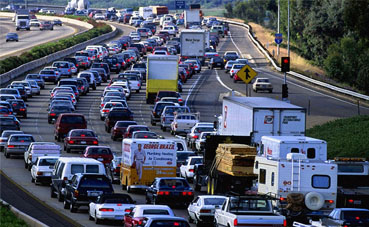
\includegraphics[scale=0.75]{traffic.jpg}
	\end{figure}

\paragraph{}
\emph{Traffic Flow Simulator} tiene como objetivo principal ser una herramienta útil que facilite la visualización de la simulación de tráfico en base a un modelo lógico, de forma que permita evaluar de manera clara las diferentes alternativas a situaciones concretas, permitiendo al usuario recrear dichas situaciones mediante la interacción con la herramienta teniendo en cuenta puntos importantes como son la congestión de las vías o los comportamientos de conducción, de forma que se pueda mejorar el flujo de tráfico en las vías urbanas. El segundo objetivo de la herramienta es posibilitar el uso de mapas de carreteras reales dentro del simulador.

\paragraph{}
El flujo de tráfico de vehículos es un sistema complejo y difícil de modelar y medir, ya que en este se ven involucradas multitud de variables dependientes unas de otras, entre las que destacan los problemas de movilidad, los cambios de sentido, las rotondas, los tiempos de semaforización, las obras en la calzada, los accidentes de tráfico y otras variables sin contar con el factor humano y las condiciones atmosféricas.

\paragraph{}
Este simulador posibilitará realizar simulaciones de tráfico sobre distintas distribuciones de redes viarias, teniendo en cuenta los diferentes perfiles de conductores que podemos encontrarnos día a día en la carretera. Así mismo, el usuario podrá personalizar las distintas variables que influirán en la simulación de forma que pueda recrear los escenarios que desee.

\paragraph{}
La parte visual estará compuesta por un entorno pasivo que no afectará al tráfico y otro activo que afectará directamente al tráfico como son semáforos, peatones y diferentes señales. 
